% DRAFT of the preprint body (2026-11-04). Not compiled yet: LaTeX is not installed in this environment.
% Claims and their evidence are in outline.md (C1--C8). The author rewrites the wording; every number
% here comes from a file named in outline.md or from the CSV/JSON files in build/ and was re-checked
% on 2026-11-04. Lines starting with "% TODO" or "% CHECK" are open items for the author.
\documentclass[11pt]{article}
\usepackage[utf8]{inputenc}
\usepackage{amsmath}
\usepackage{graphicx}
\usepackage{booktabs}
\usepackage[numbers]{natbib}
\usepackage{hyperref}
\graphicspath{{../}}

\title{Bit-exact spiking neurons on a low-cost FPGA:\\ verifying a fixed-point LIF model against hardware}
\author{TODO: authors and affiliations}
\date{TODO}

\begin{document}
\maketitle

\begin{abstract}
We describe a leaky integrate-and-fire (LIF) neuron and a 256-neuron network implemented on a low-cost FPGA (Tang Nano 20K, Gowin GW2AR-18), and we compare the hardware with a Python reference model bit for bit.
The model uses signed Q8.8 fixed-point state, saturating additions and shift-based time constants, so no multiplier is needed.
A single neuron matched the model on the board in every sampled step, with no mismatch: 60,000 samples in three hand-picked parameter sets and 2,023,200 samples in a sweep of 2,248 parameter sets.
A time-multiplexed network of 256 neurons with event-driven synapses, controlled over a UART link, matched the model on every reply of a 682-frame command flow, and on five excitation/inhibition conditions that include the spikes of every neuron in the first 512 steps.
The full design uses 12\% of the logic and 97\% of the block RAM, and meets timing at 41.38~MHz against a 27~MHz clock.
We report the verification method, including mutation tests that show the checkers can fail, and the limits we found: a UART bridge that drops bytes in long bursts, a decoder without a time-out, and a spike trace that covers only the first 512 steps.
We make no claim about biological validity; the hardware is validated against the model only.
\end{abstract}

\section{Introduction}
Spiking neuron models are small enough to run on inexpensive FPGAs, and many FPGA designs for spiking networks exist \citep{szczerek2025}.
A hardware result is only useful for model-based experiments if one can say how it differs from the model.
Several reports we read validate a design by task accuracy or by functional agreement with a simulator.
% CHECK: this is based on Fan 2025 and Gautam 2025 (notes in docs/papers/notes); do not generalise beyond what was read.
Here we ask for more: the hardware state after every step equals the state of a reference model, with zero differences.
This turns a check of the hardware into a yes-or-no test that a single flipped bit can fail.

Related FPGA work includes a time-multiplexed accelerator whose integer LIF neurons are checked against a bit-accurate software model on an image-classification task \citep{ansari2026}, a systolic simulator that updates only the neurons that spike \citep{cheung2009}, and an open-source framework for low-end FPGAs with 8-bit quantisation \citep{fan2025}.
% CHECK: Ansari 2026 is an arXiv preprint (arXiv:2608.00595); cite as preprint. Cheung 2009 and Fan 2025: read in full, see docs/papers/notes.
These designs target other boards and tasks, and their numbers are not directly comparable with ours.
% TODO: state the gap in the author's own words after reading the full list in docs/papers/README.md (groups 2 and 3).

This paper makes three contributions.
(i)~An exact specification of a fixed-point LIF neuron and of a network update rule that does not depend on the order in which spikes arrive.
(ii)~A verification method in which the model is the specification, checked in simulation, with mutation tests, and on the board, step by step.
(iii)~A 256-neuron, UART-controlled network on a low-cost board, with the resources it needs and the limits we measured.

The network is built for excitation/inhibition (E/I) perturbation experiments \citep{brunel2000}.
% CHECK: Brunel 2000: full text not read (metadata only). Keep this sentence at the level of "the class of network studied", add no claim about its results.
We include one such experiment as a demonstration that the hardware and the model agree under changing E/I balance.

\section{Model}
\label{sec:model}
\subsection{Single neuron}
The neuron is discrete in time \citep[for continuous-time LIF models see][]{gerstner2002}. Each step updates a membrane potential $V$ and a synaptic current $I$:
\begin{align}
I[t+1] &= I[t] - \left(I[t] \gg k_s\right) + x[t], \\
V[t+1] &= V[t] + \left((V_{\mathrm{rest}} - V[t]) \gg k_m\right) + I[t+1],
\end{align}
where $x[t]$ is the input of the step.
If the neuron is not refractory and $V[t+1] \ge \theta$, it emits a spike, $V$ is set to $V_{\mathrm{reset}}$, and the neuron is refractory for $\mathit{refrac}$ steps.
While it is refractory, $V$ is held at $V_{\mathrm{reset}}$ and $I$ keeps integrating.
The parameters are $\theta$, $V_{\mathrm{reset}}$, $V_{\mathrm{rest}}$, $k_m$ and $k_s$ (0--15), and $\mathit{refrac}$ (0--7).
A right shift by $k$ divides by $2^k$, so the time constants are $\Delta t/\tau = 2^{-k}$.

\subsection{Number format}
$V$ and $I$ are signed 16-bit numbers in Q8.8 format (raw value = real value $\times 256$).
Three rules fix the arithmetic exactly:
\begin{itemize}
\item Every addition saturates to $[-32768,\,32767]$ after each addition, from left to right. Nothing wraps.
\item Right shifts are arithmetic (they round toward $-\infty$).
\item $V_{\mathrm{rest}} - V$ is computed with more than 16 bits before the shift, because the difference of two 16-bit values may need 17 bits.
\end{itemize}
Saturation avoids a strong excitatory input turning into a strong inhibitory one by wrapping. A logical shift would turn a decaying negative potential into a large positive one. Both are easy to get wrong in hardware, and both are caught by the checks in Section~\ref{sec:verify}.
The reference is a short Python function (\texttt{model/fixed.py}); the hardware must match it exactly.

\subsection{Network}
All neurons share one parameter set. For neuron $i$ at step $t$ the input is
\begin{equation}
x_i[t] = \mathrm{sat}\!\left(\sum_j \left(W_{ji} \ll w_{\mathrm{shift}}\right) s_j[t-1] \;+\; \mathrm{ext}_i\right),
\end{equation}
where $W$ is a matrix of signed 8-bit weights, $w_{\mathrm{shift}}=2$ is a global scale, $s_j[t-1]$ is the spike of neuron $j$ in the previous step, and $\mathrm{ext}_i$ is a constant external input.
The sum over spikes is exact, the external input is added to it, and the total saturates once.
This differs from the single-neuron rule on purpose: the hardware processes spikes as events, in an order that depends on arrival, so saturating after each addition would make the result depend on that order.
An exact sum followed by one saturation does not. A spike at step $t$ reaches the inputs at step $t+1$.

\section{Hardware}
\label{sec:hardware}
\subsection{Board and link}
The target is a Tang Nano 20K with a Gowin GW2AR-18 device and a 27~MHz clock. A UART link at 115,200 baud connects it to a PC. The toolchain is open source (yosys, nextpnr-himbaechel, openFPGALoader).
Frames have the form \texttt{[0xA5][cmd][len][data][checksum]}, with an additive checksum.
The decoder on the FPGA rejects a frame with a bad checksum or an out-of-range value, and counts accepted and rejected frames. It refuses every command while it is busy sending a reply, copying a payload or running the network.

\subsection{Single neuron}
One neuron step takes one clock cycle: the update is a combinational circuit, and the state is held in registers.
Each step writes $\{$spike, $V\}$ (17 bits) to a record memory of 1,024 steps in block RAM. The host reads the records back in batches.
Each run starts from rest ($V=0$, $I=0$, no refractory time), the same initial condition as the model.

\subsection{Network}
\label{sec:network-hw}
The network of $N=256$ neurons uses one copy of the neuron circuit, shared in time: one step takes $N$ neuron updates followed by the synapse phase.
All memories (neuron state, external input, weights, spike flags and synaptic accumulators) have one write port and one synchronous read port, so the synthesis tool maps them to block RAM.
The same memories written as arrays become flip-flops, which needs about 45,000 cells at $N=256$ and does not fit.
Synaptic input is event driven: when neuron $j$ spikes, its weight row is added to an accumulator for the next step.
Two accumulators alternate, one read while the other is written.
Both phases are pipelined with a one-cycle read latency. The read order keeps consecutive reads on different neurons, so the pipeline never reads a value that is still being written.

The board does not keep the full state of every step: at $N=256$ and 1,024 steps, that would need about 4.4~Mbit, and the block RAM holds about 828~Kbit.
The board keeps a 16-bit spike count and a last-step snapshot of every neuron ($33N$ bits), and the spikes of every neuron for the first 512 steps of a run (one bit per neuron and step, 128~Kbit), returned seven steps per frame.
The membrane potential is therefore compared only at the last step, which is the main limit of the network verification (Section~\ref{sec:limits}).

\section{Verification}
\label{sec:verify}
The model is the specification, and a difference of one bit is a failure.
The verification has four layers.

\paragraph{Simulation.}
The single neuron was checked with cocotb and Icarus Verilog against the model: 10,110 combinational cases and 15 traces of 500 steps each.
The network core was checked against the model for $N=16, 64, 256$ over 3,200, 12,800 and 51,200 records, and the full design was checked at the byte level through the UART pins for the same sizes (for $N=256$, 682 frames).

\paragraph{Mutation tests.}
A checker that has never failed does not show that it can fail.
Each checker was therefore run on deliberately broken copies of the design, and each broken copy was caught.
Examples: replacing the arithmetic shift with a logical shift (single neuron); a weight shift of 3, a missing last target, no spike delivery, and a write to the wrong accumulator (network core); swapped input bytes, an off-by-one range check and a wrong read-modify-write timing (full design); a changed bit order, a step address off by one, a limit of 513 instead of 512 steps and a limit of eight instead of seven steps per frame (spike trace); and a status read that ignores the busy signal (busy test).
The byte-level testbench of the single neuron exposed a real design error early: a first version sent a second run while the previous reply was still being sent, which overwrote the record memory. The busy rule of Section~\ref{sec:hardware} is the fix.

\paragraph{Board, single neuron.}
The host writes the parameters, confirms them with a status read, runs the neuron, reads every step's $V$ and spike back and compares them with the model.

\paragraph{Board, network.}
The host sends the full command flow of 682 frames (70,168 bytes in, 1,892 bytes out) and compares every reply byte with the model's prediction.
The flow contains deliberately invalid frames, which must be refused without changing any state.
The E/I conditions are compared in the same way: spike counts, last-step snapshot and the spikes of the first 512 steps against the full model.

\paragraph{Not possible: netlist simulation.}
The block-RAM simulation models that come with the installed toolchain are empty, so a netlist simulation cannot run.
The board result is therefore the evidence that the synthesised design is functionally correct.

\section{Results}
\label{sec:results}
\subsection{Single neuron on the board}
Table~\ref{tab:m2} shows three parameter sets with 20 constant input currents each (from $-0.1$ to $0.375$) and 1,000 steps per input.
All 60,000 samples matched the model, and the error counter of the board stayed at zero.
Figure~\ref{fig:trace} shows the first 100 steps of one run, and Figure~\ref{fig:fi} the f--I points of the board against the model.

\begin{table}[t]
\centering
\caption{Single neuron: board against model. Values are real numbers; the Q8.8 raw value is the real value times 256.}
\label{tab:m2}
\begin{tabular}{lrrrrrrrr}
\toprule
Set & $\theta$ & $V_{\mathrm{rest}}$ & $V_{\mathrm{reset}}$ & $k_m$ & $k_s$ & refrac & Samples & Mismatches \\
\midrule
A & 2.0 & $-0.25$ & 0 & 4 & 3 & 2 & 20,000 & 0 \\
B & 0.5 & 0.25 & $-0.5$ & 0 & 0 & 0 & 20,000 & 0 \\
C & 2.0 & 0 & $-0.5$ & 15 & 15 & 7 & 20,000 & 0 \\
\bottomrule
\end{tabular}
\end{table}

\begin{figure}[t]
\centering
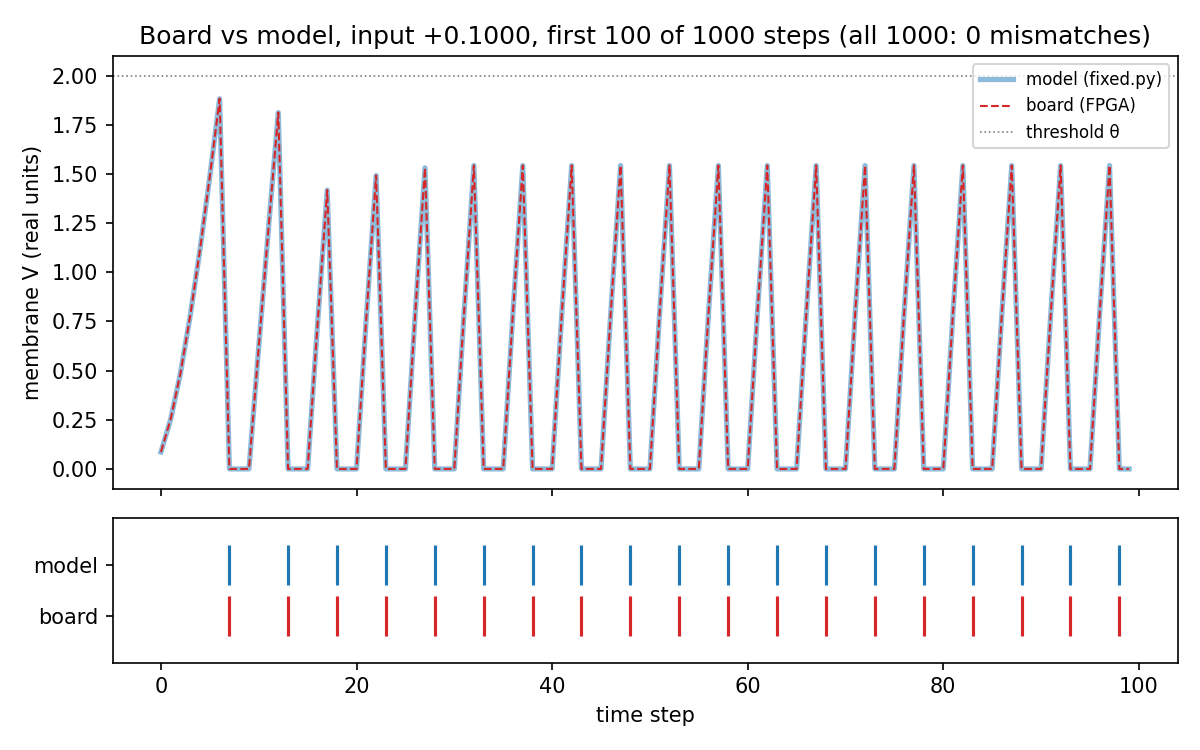
\includegraphics[width=\linewidth]{m2_trace_board_vs_model.png}
\caption{Membrane potential and spikes of parameter set A, board against model, first 100 of 1,000 steps. TODO: check the caption against \texttt{host/plot\_trial.py}.}
\label{fig:trace}
\end{figure}

\begin{figure}[t]
\centering
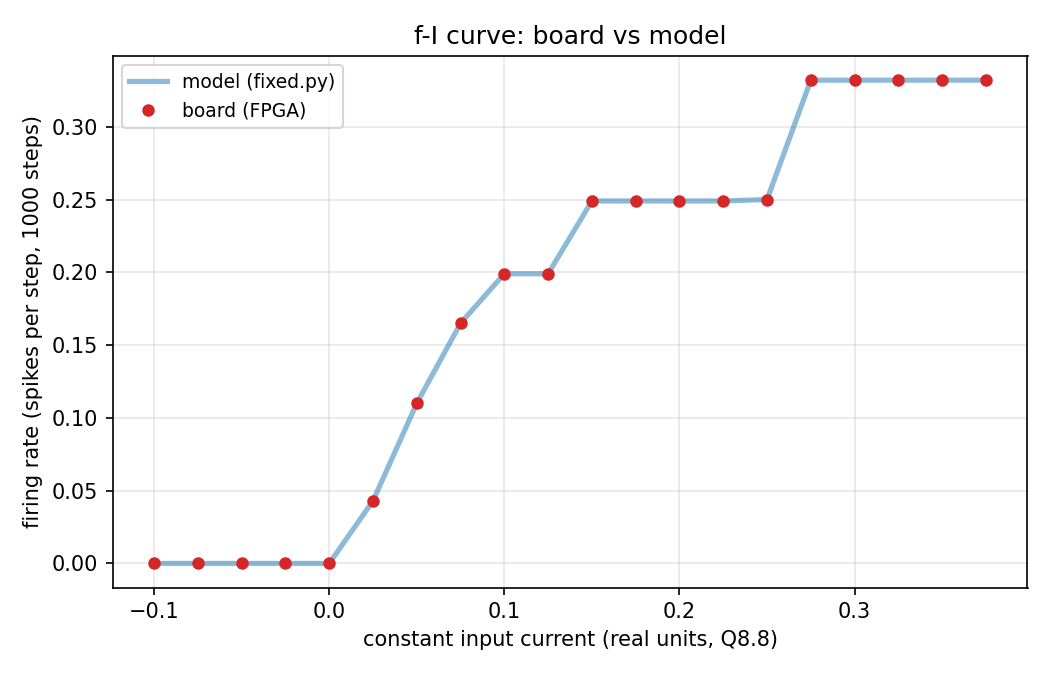
\includegraphics[width=0.8\linewidth]{m2_fi_board.png}
\caption{f--I curve: board points and model. The staircase comes from the refractory period and the dead zone of the arithmetic shift.}
\label{fig:fi}
\end{figure}

The fixed-point and floating-point models agree in shape, with a largest difference of 0.027 spikes per step (\texttt{docs/fi\_curve.png}).
% TODO: decide whether to include docs/fi_curve.png as a third figure.

\subsection{Parameter sweep}
Table~\ref{tab:sweep} covers every legal value of $k_m$, $k_s$ and $\mathit{refrac}$, and 200 random parameter sets.
Each set ran three constant inputs ($-0.2$, 0.1, 0.4) for 300 steps.
Across both sweeps, 2,023,200 samples matched with no mismatch, no failed read and no refused request.
Sets without spikes (24 grid, 5 random) are included on purpose: a silent neuron has to match the model too.

\begin{table}[t]
\centering
\caption{Parameter sweep on the board. Grid: $\theta=1.0$, $V_{\mathrm{reset}}=-0.25$, $V_{\mathrm{rest}}=0.125$ fixed. Random: all six parameters drawn at random (seed 20261103).}
\label{tab:sweep}
\begin{tabular}{lrrrrrr}
\toprule
Sweep & Sets & Samples & Mismatches & Failed reads & Sets with spikes \\
\midrule
Grid & 2,048 & 1,843,200 & 0 & 0 & 2,024 \\
Random & 200 & 180,000 & 0 & 0 & 195 \\
\bottomrule
\end{tabular}
\end{table}

\subsection{Network on the board}
The 682-frame flow at $N=256$ gave 1,892 reply bytes, all identical to the model, in 45.7~s.
Five E/I conditions then ran on the board, each with 745 frames and the spikes of the first 512 steps: $(f_{\mathrm{inh}}, w_{\mathrm{inh}}, w_{\max}, e_{\max}) = (0.2, 1, 10, 30)$, $(0.5, 1, 10, 30)$, $(0.5, 0.5, 10, 30)$, $(0.5, 2, 10, 30)$ and $(0.3, 1.5, 20, 10)$.
All five matched the full model bit for bit.

\subsection{E/I demonstration (model)}
\label{sec:ei}
The demonstration uses random networks of 256 neurons with a connection probability of $8/N$, a fraction $f_{\mathrm{inh}}$ of inhibitory sources, and excitatory weights drawn from $[0, w_{\max}]$ with $w_{\max}=10$.
Each neuron has a constant external input drawn from $[0, e_{\max}]$ (Q8.8 raw) with $e_{\max}=30$. Each run has 600 steps, and the first 100 are discarded.
Table~\ref{tab:ei} gives the mean firing rate in spikes per step and per neuron. It falls monotonically as $f_{\mathrm{inh}}$ rises, and the share of silent neurons rises.
A full sweep of 504 runs, which also varied $w_{\mathrm{inh}}$, $w_{\max}$ and $e_{\max}$, was monotone in all 24 parameter combinations (tolerance 0.005).
Only the five conditions listed above also ran on the board.
We had to lower $w_{\max}$ from 60 to 10: with 60, the network was either silent or at the refractory limit of 1/3 spikes per step, and the external input no longer mattered.
For $f_{\mathrm{inh}}<0.2$ most neurons sit near that limit, so the useful range of the perturbation is about 0.2 to 0.6.

\begin{table}[t]
\centering
\caption{Mean firing rate against $f_{\mathrm{inh}}$ ($w_{\max}=10$, $e_{\max}=30$, $w_{\mathrm{inh}}=1$): mean over three random networks (minimum--maximum in brackets), and share of silent neurons. Model only. Rates are per time step, not in Hz.}
\label{tab:ei}
\begin{tabular}{rcc}
\toprule
$f_{\mathrm{inh}}$ & Mean rate (min--max) & Silent neurons \\
\midrule
0.0 & 0.316 (0.313--0.319) & 0.00 \\
0.1 & 0.291 (0.284--0.294) & 0.01 \\
0.2 & 0.249 (0.242--0.253) & 0.02 \\
0.3 & 0.210 (0.201--0.217) & 0.07 \\
0.4 & 0.175 (0.171--0.181) & 0.13 \\
0.5 & 0.149 (0.146--0.154) & 0.19 \\
0.6 & 0.123 (0.120--0.130) & 0.26 \\
\bottomrule
\end{tabular}
\end{table}
% TODO: add docs/ei_rate_vs_finh.png as a figure instead of, or beside, the table.

\subsection{Link limits}
The USB--UART bridge on the board lost bytes in long unpaced bursts: a single write of 96 or 128 bytes returned only 66 bytes in a loopback test, while 16-byte chunks paced to the line rate all came back.
The host therefore sends in 16-byte chunks at line speed, and waits for the full reply of a frame before it sends the next one.
A run takes no reply, so the host waits for a time computed from the number of steps: in the worst case a step takes $N+N^2+2N$ clock cycles.

\section{Resources and scaling}
\label{sec:resources}
Table~\ref{tab:res} gives the place-and-route result of the full design at $N=256$.
A single neuron needs about 274 LUTs.
The network core alone (yosys) came to 1,382, 1,343 and 1,457 cells at $N=16, 64, 256$: its size is almost independent of $N$, because the state and the weights are in block RAM.
Block RAM is what limits the design: the weight matrix alone is $N^2 \times 8$ bits (512~Kbit), and the spike trace takes eight more blocks. With 45 of 46 blocks used, we cannot add a feature without first freeing memory.
The weight matrix grows as $N^2$: for $N=512$ it would be 2~Mbit, more than the roughly 828~Kbit of block RAM on the chip.
% CHECK: the $N=512$ figure is arithmetic from the N^2 weight matrix, not a built or measured design. Keep it or remove it.

\begin{table}[t]
\centering
\caption{Full design at $N=256$ (nextpnr-himbaechel, GW2AR-18).}
\label{tab:res}
\begin{tabular}{lrr}
\toprule
Resource & Used & Available \\
\midrule
LUT4 & 2,536 & 20,736 (12\%) \\
Flip-flops & 1,315 & 15,552 (8\%) \\
Block RAM & 45 & 46 (97\%) \\
Maximum clock & 41.38~MHz & 27~MHz target, met \\
\bottomrule
\end{tabular}
\end{table}

\section{Limitations}
\label{sec:limits}
\begin{itemize}
\item \textbf{Biology.} The hardware is validated against the model only. The E/I demonstration uses synthetic random networks, weights that are not calibrated against data, and rates per time step, not in Hz. We draw no conclusion about neural tissue.
\item \textbf{Membrane potential in the network.} The board compares spikes for the first 512 steps, and $V$ only at the last step. An intermediate $V$ would need a run of that length from rest for each step. A run of more than 512 steps keeps only the counts and the last snapshot after step 512.
\item \textbf{No netlist simulation.} The block-RAM models of the installed toolchain are empty. The synthesis tool prints range warnings for some memory mappings. The board result is our evidence that these do not matter, but it is a test of the cases we ran, not a proof.
\item \textbf{Parameter space.} All neurons share one parameter set, there is no noise source, and the grid sweep fixes $\theta$, $V_{\mathrm{reset}}$ and $V_{\mathrm{rest}}$ (the random sweep covers them).
\item \textbf{Protocol.} The additive checksum does not detect swapped bytes. The decoder has no time-out, so a corrupted length field can misalign the frame stream. The board has no reset command, so its counters persist until the bitstream is reloaded, and the command-flow test must start from a freshly loaded board.
\item \textbf{Draft decisions.} The protocol, the weight scale $w_{\mathrm{shift}}$ and the choice of the E/I test network are our own decisions and are not tuned or compared with alternatives.
\item \textbf{Samples.} Each E/I data point uses three random networks and one external-input sample. The board ran five conditions of the 24.
\end{itemize}

\section*{Availability}
% TODO: repository link (decide before submission). The repository contains the model, RTL, testbenches, host scripts and the raw results in build/.

\section*{AI-assisted development}
This project was developed with Claude Code. Design decisions, the verification method, and the accept/reject judgments are the author's. See \texttt{docs/DECISIONS.md}.
% CHECK: align this statement with README.md and with the Research Square AI-use rules before submission.

\bibliographystyle{unsrtnat}
\bibliography{references}

\end{document}
